\documentclass[]{beamer}


%\usetheme{Darmstadt}
 
\usepackage[T1]{fontenc}
\usepackage[utf8]{inputenc}
\usepackage{url}

\usepackage{multirow}
%\usefonttheme{default} % default family is serif
%\usepackage{fontspec}
%\setmainfont{Liberation Serif}


\usepackage{amsmath, amssymb}
%\usepackage{varwidth}% http://ctan.org/pkg/varwidth
\usepackage{amsmath}
\usepackage{mathtools}
\usepackage{tikz}

\usepackage{breqn}

\usetikzlibrary{calc,tikzmark,arrows,shapes,backgrounds}
%\usetikzlibrary{positioning, fit, arrows.meta, shapes}
\usetikzlibrary{fit, arrows.meta, shapes}

% used to avoid putting the same thing several times...
% Command \empt{var1}{var2}
%\newcommand{\empt}[2]{$#1^{\langle #2 \rangle}$}
\newcommand{\empt}[2]{$#1^{( #2 )}$}



\setbeamertemplate{footline}[frame number]
%%\setbeamertemplate{headline}{Magister en estadística - PUCV}
 

\usetikzlibrary{arrows.meta}



\title{Modelos Lineales para Clasificación}
\subtitle{Modelos para Respuesta Ordinal}
\author{Juan Zamora O.}
%\institute{Pontificia Universidad Católica de Valparaíso}
\date{}


%%% LOGO DE LA PAGINA INICIAL
\titlegraphic{
	\begin{tikzpicture}[overlay,remember picture]
		\node[opacity=0.8,below=0.3cm] at (current page.center){		
    			
\includegraphics[width=4cm]{logo_ies}
		};
	\end{tikzpicture}
}
%%% END OF LOGO




%%% LOGO DE CADA LAMINA
\logo{
	\begin{tikzpicture}[overlay,remember picture]
		\node[opacity=0.4,right=1.2cm, above=0.12cm] at (current page.south west){		
    			
\includegraphics[width=2cm]{logo_ies}
		};
	\end{tikzpicture}
}
%%% END OF LOGO



\begin{document}

\begin{frame}[noframenumbering,plain]
    \titlepage
\end{frame}

\begin{frame}{Modelos con respuestas ordinales}
	En esta parte del Curso, revisaremos problemas en que las categorias 
	de la respuesta en el problema de regresión están ordenadas\\~\ 
	
	Modelos en donde 
	Las respuestas tienden a tomar cateogrías más altas o más bajas a 
	medida que el valor de una covariable se incrementa\\~\

	Es posible explotar información del ordenamiento natural de las 
	categorías y así obtener un modelo más parsimonioso que el multinomial
\end{frame}

\begin{frame}{Modelos con respuestas ordinales}{Errores de modelamiento comúnes }
	Uso de modelos clásicos ignorando que la respuesta es ordinal. Esto genera 
	una interpretación deficiente de los resultados.\\~\ 

	Otra manera de abordar este tipo de problemas es mediante el uso de 
	regresión binaria sobre una versión colapsada de las categorías. El 
	problema en este caso es la pérdida de información.

\end{frame}

\begin{frame}{Modelos con respuestas ordinales}{Problemas de ejemplo }
	\begin{itemize}
		\item Recuperación de pacientes según calidad de vida (Excelente, Buena, Suficiente, Pobre)
		\item Dolor (Ninguno, Leve, Considerable, Severo)
		\item Inclinación política (Extrema izquierda, Izquierda moderada, Moderado, Derecha moderada, Extrema derecha)
		\item Gasto de una Institución (Muy bajo, Medio, Muy alto)
		\item Categorización de una variable ordinal. Indice de masa corporal (BMI=peso/altura): $(<18.5, 18.5-25,25-30,>30)$ para (Bajo peso, Peso normal, Sobrepeso )
	\end{itemize}

\end{frame}

\section{El problema ordinal}
\begin{frame}
	\frametitle{El problema ordinal}	

	Sea $c$ el número de categorías de la variable respuesta $Y$. A su vez 
	las probabilidades de  la respuesta satisfacen $\prod_{i=1}^c\pi_i=1$\\~\ 

	El foco está en modelo $P(y=j),\ j=\{1,2,\ldots ,c\}$, que depende de las variables explicativas $\mathbf{x}$ \\~\  

	Cuando todas las covariables son discretas, el conjunto de datos puede ser 
	agrupado en forma de conteo en las $c$ categorias de $Y$ para cada 
	configuración de las variables explicativas

\end{frame}

\iffalse
\begin{frame}
	\frametitle{Estrategia de modelamiento}

	Una forma de modelar respuestas binarias es comenzar desde modelos binarios.
	Es decir, las categorías ordenadas $1\ldots c$ son transformadas a una 
	respuesta binaria \\~\ 


\end{frame}
\fi

\subsection{Enfoque acumulativo}

\iffalse
\begin{frame}
	\frametitle{Enfoque Acumulativo}
	Enfoque más sencillo considera una división entre categorias $r$ y $r+1$, 
	produciendo las  categorias de respuesta agrupadas $\{1,\ldots , r\}$ y $\{r+1,\ldots , c\}$.\\~\
	
	El \textbf{Enfoque Acumulativo} usa estos agrupamientos, considerando la variable
	binaria $y_r=1$ si $Y\leq r$ e $y_r=0$ si $Y>r$. Es decir 	

	$$
	[1,\dots ,r|r+1,\ldots , c]\ y_r=
	\begin{cases}
        1, & Y \in \{1,\ldots , r\}\\
        0, & Y \in \{r+1,\ldots , c\} 
    \end{cases}
	$$

	El modelo de respuesta binaria resultante es
	$$P(Y\leq r|\mathbf{x})=F(\mathbf{x}^T\beta_r),\ r=1\ldots ,c-1$$


\end{frame}
\fi 


\begin{frame}{Modelo Acumulativo Simple}
	Una forma simple y muy usada es aquella que se deriva del supuesto que
	las categorías observadas en $Y$ representan una versión discreta de un modelo	de regresión para una variable continua 

	$$\widetilde{Y}=\pmb{x}^T\pmb{\beta}+\epsilon $$

	Por lo tanto $Y=r \Leftrightarrow \tau_{r-1}<\widetilde{Y}\leq \tau_{r}$. Siendo 
	$(\tau_{0},\tau_{1},\ldots , \tau_{c})$ puntos de corte en la escala latente. Por lo tanto, 
	$$P(Y\leq r|\pmb{x})=P(\widetilde{Y}\leq \tau_{r}|\pmb{x})=F(\tau_{r} - \pmb{x}^T\pmb{\beta})$$
		
	Luego el modelo queda especificado como $$F^{-1}(P(Y\leq r|\pmb{x}))=\tau_{r} - \pmb{x}^T\pmb{\beta}$$
\end{frame}

\begin{frame}
	Por ejemplo, cuando $F$ es la función acumulada de la distribución logística, su inversa $F^{-1}$ 
	es la función \textit{logit}. Por lo tanto, el \textbf{modelo acumulativo logit} consiste en 
	$$logit(P(Y\leq r|\pmb{x}))=\log\left(\frac{P(Y\leq r|\pmb{x})}{P(Y> r|\pmb{x})}\right)=\tau_{r} - \pmb{x}^T\pmb{\beta}$$

	El signo que acompaña a $\pmb{x}^T\pmb{\beta} $ puede ser positivo o negativo. Por ejemplo, el método polr de la librería MASS supone esta parametrización (VGAM usa signo positivo).\\~\ 

	Otro modelo similar se genera cuando $F$ es la función de densidad acumulada de una normal standard. 
	Este modelo se denomina modelo acumulativo \textit{probit} y funciona bien cuando el modelo de regresión
	subyacente tiene una $\widetilde{Y}\sim \mathcal{N}(0,1)$
	

\end{frame}

\begin{frame}
	\frametitle{}

	Por ejemplo, para una respuesta con 4 niveles.% cuyo modelo de regresión subyacente con una covariable que
	
	%además 
	Supone una distribución normal standard para $\widetilde{Y}$:
	\begin{tikzpicture}[remember picture, overlay]
        \node[above=1.7cm] at (current page.south) 
        {
            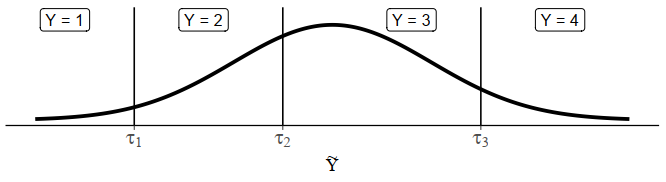
\includegraphics[width=0.9\textwidth]{ordinal_model_classes_cumulative.png}
        };
        %\node[below=-1cm,font=\fontsize{5pt}{5pt}\selectfont] at (current page.south)  {Extracted from \url{https://web.stanford.edu/class/cs224n/}};
    \end{tikzpicture}


\end{frame}

\begin{frame}
	\frametitle{Conclusiones generales}
	Usualmente, un coeficiente $\beta_j>0$ se interpreta como un efecto positivo de esa covariable 
	en la probabilidad de que $Y$ tome determinada categoría.\\~\
	
	A menudo se hace una interpretación de la variable latente (no observada). Sin embargo, el modelo 
	resultante puede ser usado sin referencia alguna a la variable latente.\\~\  

	Debido a la derivación del modelo de regresión latente, el efecto de $\pmb{x}$ no depende de la 
	categoría, es decir es un \textbf{efecto global}.\\~\ 

	El modelo más usado es el logit acumulado o también llamado modelo de probabilidades 
	proporcionales (\textit{proportional odds})
\end{frame}

\subsection{Ejemplos}


\begin{frame}
	\frametitle{Ejemplo: Discapacidad mental}
	% 
	Discapacidad intelectual, medida en una escala de 4 puntos, con eventos de la vida y status socioeconómico. Comprende 40 observaciones de un estudio con personas.
	
	Respuesta categorizada en  `Well`, `Mild symptom formation`, `Moderate symptom` y `Impaired`
	
	% latex table generated in R 4.2.2 by xtable 1.8-4 package
% Sat May 27 05:38:03 2023
\begin{table}[ht]
\centering
\begin{tabular}{cccc}
  \hline
 Subject & Mental.Impairment & Life.Events & SES \\ 
  \hline
1 & Well &   1 & high \\ 
2 & Well &   9 & high \\ 
3 & Mild &   4 & high \\ 
... & ... &  ... &  ... \\
39 & Moderate &   2 & low \\ 
40 & Impaired &   0 & high \\ 
 
   \hline
\end{tabular}
\end{table}
\end{frame}

\begin{frame}
	\frametitle{Modelo}
	
	$$logit[\widehat{P}(y_i\leq j)] =\alpha_j + \beta_{1}x_{i1}+ \beta_{2}x_{i2} $$
	
	\begin{itemize}
		\item 	$x_{1}$ corresponde a la variable \textsc{Life.Events} que es una medida compuesta de la cantidad e importancia de eventos ocurridos en la vida de un sujeto.
	
	   \item $x_{2}$ \textsc{SES} indica el \textit{status} socieconómico como alto (SES=1) o bajo (SES=0). 
	
	\end{itemize}

\end{frame}


\begin{frame}
	\frametitle{Parámetros ajustados}
	
	

% latex table generated in R 4.2.2 by xtable 1.8-4 package
% Sun May 28 19:39:43 2023
\begin{table}[ht]
\centering
\begin{tabular}{rrrrr}
  \hline
 & Estimate & Std. Error & z value & Pr($>$$|$z$|$) \\ 
  \hline
(Intercept):1 & -0.2819 & 0.6231 & -0.4524 & 0.6510 \\ 
  (Intercept):2 & 1.2128 & 0.6511 & 1.8626 & 0.0625 \\ 
  (Intercept):3 & 2.2094 & 0.7171 & 3.0810 & 0.0021 \\ 
  Life.Events & -0.3189 & 0.1194 & -2.6699 & 0.0076 \\ 
  SEShigh & 1.1112 & 0.6143 & 1.8090 & 0.0704 \\ 
   \hline
\end{tabular}
\end{table}


Recordar que para calcular la probabilidad para cada nivel se evalua primero la expresión
$$\widehat{P}(y_i\leq j) =\frac{\exp^{\alpha_j + \beta_{1}x_{i1}+ \beta_{2}x_{i2}}}{1+ \exp^{\alpha_j + \beta_{1}x_{i1}+ \beta_{2}x_{i2}}}= \frac{\exp^{\alpha_j -0.3189x_{i1}+ 1.1112x_{i2}}}{1+ \exp^{\alpha_j -0.3189x_{i1}+ 1.1112x_{i2}}} $$

y luego se calcula $$\widehat{P}((j-1)\leq y_i\leq j)= \widehat{P}(y_i\leq j)  - \widehat{P}(y_i\leq (j-1))$$

\end{frame}


\begin{frame}
\begin{itemize}
	\item Considerando un valor fijo para \textsc{Life.Events}, en el nivel alto de \textsc{SES} las \textit{odds} estimadas de discapacidad mental para cualquier nivel dado, son $\exp^{1.1112}=3.038$ veces las \textit{odds}  estimadas para el nivel bajo de \textsc{SES}.
	
	\item Tomando el error std. podemos también identificar que el I.C. al $95\%$ para este efecto es $$exp^{1.1112\pm 1.96(0.6143)}= [0.9114,10.1272] $$

\end{itemize}	
\end{frame}

\begin{frame}
La probabilidad acumulada, comenzando en el nivel "Well", disminuye a medida que \textsf{Life.Events} aumenta, y es más alto para el nivel más alto de \textsf{SES}.
\vspace{30pt}

	\begin{tikzpicture}[remember picture, overlay]
        \node[above=0.6cm] at (current page.south) 
        {
            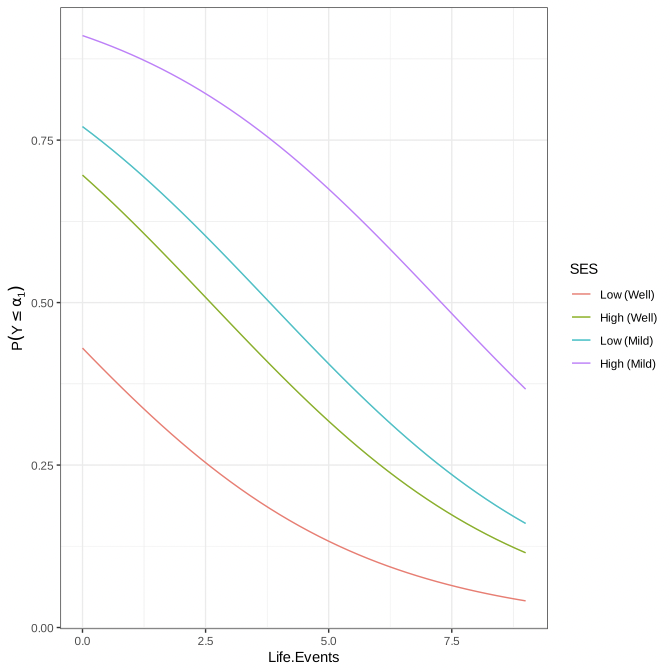
\includegraphics[width=0.45\textwidth]{mentalimpairment_well_cat_ses2.png}
        };
    \end{tikzpicture}
\end{frame}



\begin{frame}
	\frametitle{Salida para el modelo anterior con `polr`}

En este caso se usa parametrización $\alpha_j -\pmb{x}^T\pmb{\beta} $. Sin embargo, los coeficientes son los mismos.


% latex table generated in R 4.2.2 by xtable 1.8-4 package
% Sun May 28 20:28:45 2023
\begin{table}[ht]
\centering
\begin{tabular}{rrrr}
  \hline
 & Value & Std. Error & t value \\ 
  \hline
Life.Events & 0.3189 & 0.1210 & 2.6354 \\ 
  SEShigh & -1.1112 & 0.6109 & -1.8191 \\ 
  Well$|$Mild & -0.2819 & 0.6423 & -0.4389 \\ 
  Mild$|$Moderate & 1.2128 & 0.6607 & 1.8357 \\ 
  Moderate$|$Impaired & 2.2094 & 0.7210 & 3.0644 \\ 
   \hline
\end{tabular}
\end{table}

\end{frame}


%%%%
%%%% Otro ejemplo
\begin{frame}
	\frametitle{Ejemplo: Estudio de lesión de rodilla}
	% p241 - tutz
	Reporte de dolor post-tratamiento en una escala de 5 puntos.
	
\begin{table}[]
\begin{tabular}{lccccc}
                     & \textbf{Sin dolor} &    &  $\longrightarrow $  &    & \textbf{Dolor severo} \\
                     & 1                  & 2  & 3  & 4  & 5                     \\ \hline
\textbf{Placebo}     & 17                 & 8  & 14 & 20 & 4                     \\
\textbf{Tratamiento} & 19                 & 26 & 11 & 6  & 2                     \\ \hline
\end{tabular}
\end{table}
	
\textbf{Objetivo}: Cuantificar asociación entre efecto del tratamiento y nivel de dolor
\end{frame}


\begin{frame}
	\frametitle{Modelo y parámetros ajustados}

El modelo corresponde a:	
$$logit[\widehat{P}(y_i\leq j)] =\alpha_j + \beta_{1}x_{i1}$$

donde $x_1$ corresponde a la pertenencia al grupo de placebo (\textsc{Th}=P) o tratamiento (\textsc{Th}=T).

	% latex table generated in R 4.2.2 by xtable 1.8-4 package
% Sun May 28 22:10:25 2023
\begin{table}[ht]
\centering
\begin{tabular}{rrrrr}
  \hline
 & Estimate & Std. Error & z value & Pr($>$$|$z$|$) \\ 
  \hline
(Intercept):1 & -1.4659 & 0.2742 & -5.3470 & 0.0000 \\ 
  (Intercept):2 & -0.2860 & 0.2413 & -1.1853 & 0.2359 \\ 
  (Intercept):3 & 0.6668 & 0.2488 & 2.6804 & 0.0074 \\ 
  (Intercept):4 & 2.6436 & 0.4365 & 6.0568 & 0.0000 \\ 
  ThT & 0.8932 & 0.3250 & 2.7483 & 0.0060 \\ 
   \hline
\end{tabular}
\end{table}
\end{frame}


\begin{frame}
	\begin{itemize}
		\item El efecto del tratamiento producido por el modelo es de $0.8932$ con un error std. de $0.325$. 
		\item Esto muestra un efecto en la respuesta producto de la realización del tratamiento.
		\item Además, para cualquier categoría de la respuesta, la razón de \textit{odds} acumulados entre tratamiento y placebo cumple con $$\frac{P(y_i\leq j|T)/P(y_i> j|T)}{P(y_i\leq j|P)/P(y_i> j|P)}=\exp^{0.8932}=2.443$$
	\end{itemize}

Por lo tanto, las \textit{odds} para cualquier categoría de menor dolor, en comparación con categorías más altas de la respuesta ($+$ dolor) son más altas en el grupo de \textbf{T}ratamiento.
\end{frame}

\begin{frame}
	\textbf{Calculando algunas probabilidades}
	Tomando los coeficientes resultantes para cada nivel (interceptos) junto con el coeficiente asociado a la covariable grupo, podemos calcular las siguientes probabilidades:
	
	\begin{table}[]
\begin{tabular}{lccccc}
                & \textbf{Sin dolor} &    &    &    & \textbf{Dolor severo} \\
                     & 1                  & 2  & 3  & 4  & 5                     \\ \hline
\textbf{Placebo}     & 0.1876                 & 0.2414  & 0.2318 & 0.2728 & 0.0664                     \\
\textbf{Tratamiento} & 0.3606                 & 0.2867 & 0.1791 & 0.1454  & 0.0283                     \\ \hline
\end{tabular}
\end{table}
	
	Notar como va aumentando la probabilidad de reportar un dolor más intenso para el grupo P, en contraste con la disminución de esta misma para el grupo T.
\end{frame}
%%%%%%%%%%%%%%%%
\end{document}